% Created 2015-11-23 Mon 15:57
\documentclass[9pt]{beamer}
\usepackage[utf8]{inputenc}
\usepackage[T1]{fontenc}
\usepackage{fixltx2e}
\usepackage{graphicx}
\usepackage{longtable}
\usepackage{float}
\usepackage{wrapfig}
\usepackage{soul}
\usepackage{textcomp}
\usepackage{marvosym}
\usepackage{wasysym}
\usepackage{latexsym}
\usepackage{amssymb}
\usepackage{hyperref}
\tolerance=1000
\mode<beamer>{\usetheme{Warsaw}}
\mode<beamer>{\setbeamertemplate{blocks}[rounded][shadow=false]}
\mode<beamer>{\addtobeamertemplate{block begin}{\pgfsetfillopacity{0.8}}{\pgfsetfillopacity{1}}}
\mode<beamer>{\setbeamercolor{structure}{fg=orange}}
\mode<beamer>{\setbeamercovered{transparent}}
\AtBeginSection[]{\begin{frame}<beamer>\frametitle{Topic}\tableofcontents[currentsection]\end{frame}}
\usepackage{subcaption}
\usepackage{multimedia}
\usepackage{tikz}
\usepackage{subfigure,subfigmat}
\usepackage{threeparttable}
\usetikzlibrary{shapes,arrows,shadows}
\usepackage{bm, amssymb, amsmath, array, pdfpages,graphicx}
\newcommand{\bv}[1]{\mathbf{#1}}
\newcommand{\diff}[2]{\frac{\partial #1}{\partial #2}}
\newcommand{\beq}[0]{\begin{equation}}
\newcommand{\eeq}[0]{\end{equation}}
\newcommand{\beqa}[0]{\begin{eqnarray}}
\newcommand{\eeqa}[0]{\end{eqnarray}}
\newcommand{\beqq}[0]{\begin{equation*}}
\newcommand{\eeqq}[0]{\end{equation*}}
\newcommand{\bs}[1]{\boldsymbol{#1}}
\newcommand{\ip}[2]{\langle #1, #2\rangle}
\providecommand{\alert}[1]{\textbf{#1}}

\title{Uncertainty Quantification of Low-Dimensional Models}
\author{Anthony DeGennaro \newline Scott Dawson \newline Clarence W. Rowley III \newline Princeton University}
\date{APS 68$^{th}$ Annual DFD Meeting \\ Boston, MA \\ November 2015}
\hypersetup{
  pdfkeywords={},
  pdfsubject={},
  pdfcreator={Emacs Org-mode version 7.9.3f}}

\begin{document}

\maketitle

\begin{frame}
\frametitle{Outline}
\setcounter{tocdepth}{3}
\tableofcontents
\end{frame}



% Define my settings

\graphicspath{{../Figures/}}
% Add Princeton shield logo
\addtobeamertemplate{frametitle}{}{%
\begin{tikzpicture}[remember picture,overlay]
\node[anchor=north east,yshift=2pt] at (current page.north east) {\includegraphics[height=0.7cm]{Shield}};
\end{tikzpicture}}
%


\institute{Princeton University}


\section{Introduction}
\label{sec-1}
\begin{frame}
\frametitle{Motivation}
\label{sec-1-1}

\begin{itemize}
\item Many fluid systems have uncertainties associated with them
\begin{itemize}
\item Governing parameters
\item Boundary conditions
\end{itemize}
\item Wing icing \footnote{Broeren et. al. \emph{Swept-Wing Ice Accretion Characterization and Aerodynamics}. AIAA 2013-2824.
 }\textsuperscript{,}\,\footnote{Addy, H. E. \emph{Ice Accretions and Icing Effects for Modern Airfoils}. NASA TP 2000-210031.
 }
\begin{itemize}
\item Ice shape on leading edge of airfoil varies with physical conditions
\end{itemize}
\end{itemize}
\begin{figure}[ht]
\centering
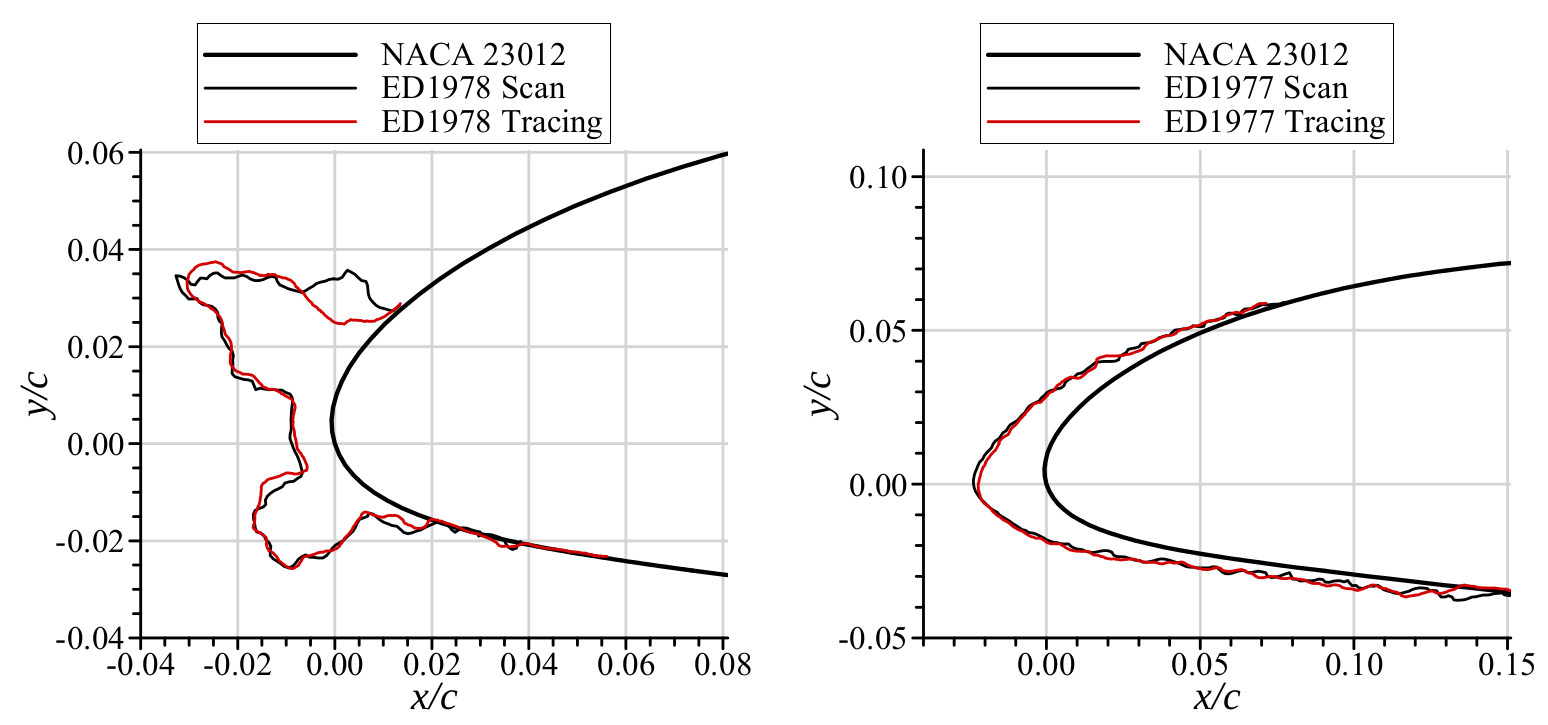
\includegraphics[width=0.7\textwidth]{SampleIceShapes} \\
\textbf{Broeren, 2013}
\end{figure}
\end{frame}
\begin{frame}
\frametitle{Motivation}
\label{sec-1-2}

\begin{itemize}
\item Many fluid systems have uncertainties associated with them
\begin{itemize}
\item Governing parameters
\item Boundary conditions
\end{itemize}
\item Airplane cargo hold fires \footnote{DeGennaro, Lohry et. al. \emph{Uncertainty Quantification for Cargo Hold Fires}. To appear at AIAA Scitech 2016.
 }
\begin{itemize}
\item Fire source location, temperature can be uncertain
\end{itemize}
\end{itemize}
\begin{figure}[ht]
\centering
\begin{minipage}[b]{0.45\linewidth}
\movie[width=0.9\textwidth,height=0.66\textwidth,poster,autostart,loop,borderwidth]{}{FireColdCenter.avi} \\
\centering
\textbf{Colder Source} \\
\end{minipage}
\begin{minipage}[b]{0.45\linewidth}
\movie[width=0.9\textwidth,height=0.66\textwidth,poster,autostart,loop,borderwidth]{}{FireHotCenter.avi} \\
\centering
\textbf{Hotter Source}
\end{minipage}
\end{figure}
\end{frame}
\begin{frame}
\frametitle{Motivation}
\label{sec-1-3}

\textbf{Goal: apply uncertainty quantification tools to low-dimensional models}
\begin{itemize}
\item Investigate statistical variations in spatial structures and dynamics
\begin{itemize}
\item POD modes, DMD modes
\item DMD eigenvalues
\end{itemize}
\end{itemize}
\textbf{Potential applications}
\begin{itemize}
\item Develop low-dimensional models accurate for range of parameter uncertainty
\item POD Galerkin models
\begin{itemize}
\item Sensitive to parametric variation/uncertainty
\end{itemize}
\end{itemize}
\end{frame}
\section{Background}
\label{sec-2}
\begin{frame}
\frametitle{Low-Dimensional Modeling}
\label{sec-2-1}

\begin{itemize}
\item Proper Orthogonal Decomposition (POD)
\begin{itemize}
\item Data compression, dominant spatial features
\item Modes are eigenvectors of the dataset covariance matrix
\item Modes describe dataset better than any other linear basis
\end{itemize}
\item Dynamic Mode Decomposition (DMD)
\begin{itemize}
\item Describe dataset as linear dynamical system
\item Spatial modes + (frequencies, growth/decay rates)
\end{itemize}
\end{itemize}
%\begin{columns}[c]
%\column{0.5\textwidth}
%   \centering
%    \textbf{Cylinder, Re = 100}
%    \movie[width=0.9\textwidth,height=0.3\textwidth,poster,autostart,loop,borderwidth]{}{CylinderRe100.mp4}
%\column{0.5\textwidth}
%   \centering
%    \textbf{POD/DMD Modes} \\
%    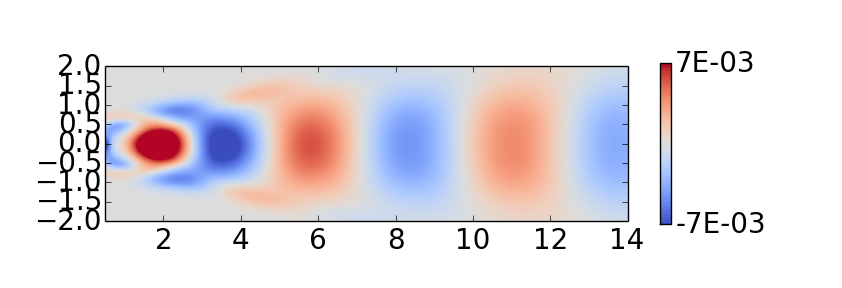
\includegraphics[width=0.9\textwidth]{CylinderRe100POD1} \\
%    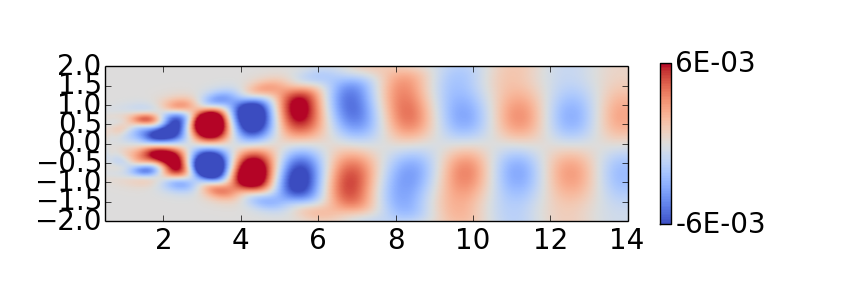
\includegraphics[width=0.9\textwidth]{CylinderRe100POD2}
%\end{columns}



\fontsize{9}\selectfont
% Define the layers to draw the diagram
\pgfdeclarelayer{background}
\pgfdeclarelayer{foreground}
\pgfsetlayers{background,main,foreground}

% Define block styles used later

\tikzstyle{basic}=[draw, fill=blue!20, text width=5em, 
    text centered, minimum height=2.5em,drop shadow]
\tikzstyle{mode} = [basic, text width=10em, fill=blue!20, 
    minimum height=4em, rounded corners, drop shadow]

% Define distances for bordering
\def\blockdist{2.3}
\def\edgedist{2.5}
\centering
\begin{tikzpicture}
    \node (Simulation) [mode]  {\movie[width=0.9\textwidth,height=0.3\textwidth,poster,autostart,loop,borderwidth]{}{CylinderRe100.mp4}\\[1em]\textbf{Cylinder: Re = 100}};
    \path (Simulation)+(4,0) node (POD1) [mode] {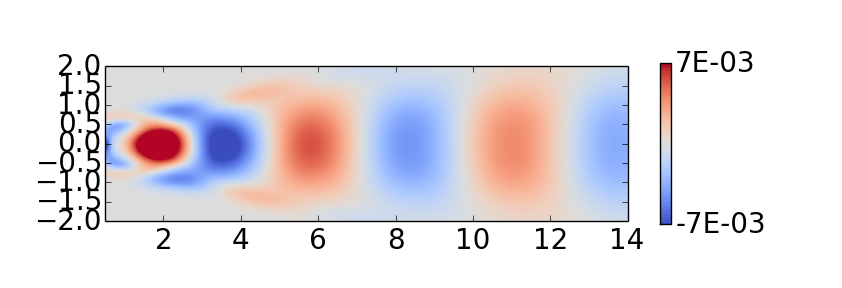
\includegraphics[width=0.9\textwidth]{CylinderRe100POD1}\\[1em] 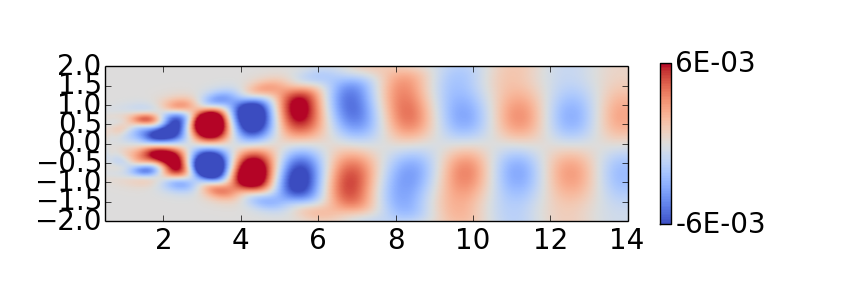
\includegraphics[width=0.9\textwidth]{CylinderRe100POD2}\\[1em]\textbf{POD/DMD Modes}};

    \path [draw, ->, thick] (Simulation.east) |- node [right] {} (POD1.west);

\end{tikzpicture}
\end{frame}
\begin{frame}
\frametitle{Polynomial Chaos Expansions (PCE)}
\label{sec-2-2}

\begin{itemize}
\item Polynomial Chaos Expansions (PCE)
\begin{itemize}
\item Method for quantifying parametric uncertainty efficiently
\item Spectral method in probability space
\item Expand output in terms of basis polynomial functions of random variables
\end{itemize}
\end{itemize}
\begin{equation*}
\begin{aligned}
f(\xi) &\approx \sum_{i}^N a_i \psi_i(\xi) \\
\langle f , g \rangle &= \int_{\Gamma} f(\xi) g(\xi) \rho(\xi) d\xi \quad , \quad \langle \psi_i , \psi_j \rangle = \delta_{ij}
\end{aligned}
\end{equation}
\fontsize{9}\selectfont
% Define the layers to draw the diagram
\pgfdeclarelayer{background}
\pgfdeclarelayer{foreground}
\pgfsetlayers{background,main,foreground}

% Define block styles used later

\tikzstyle{sensor}=[draw, fill=blue!20, text width=5em, 
    text centered, minimum height=2.5em,drop shadow]
\tikzstyle{ann} = [above, text width=5em, text centered]
\tikzstyle{wa} = [sensor, text width=10em, fill=blue!20, 
    minimum height=7em, rounded corners, drop shadow]

% Define distances for bordering
\def\blockdist{2.3}
\def\edgedist{2.5}

\begin{tikzpicture}
    \node (CleanAirfoil) [wa]  {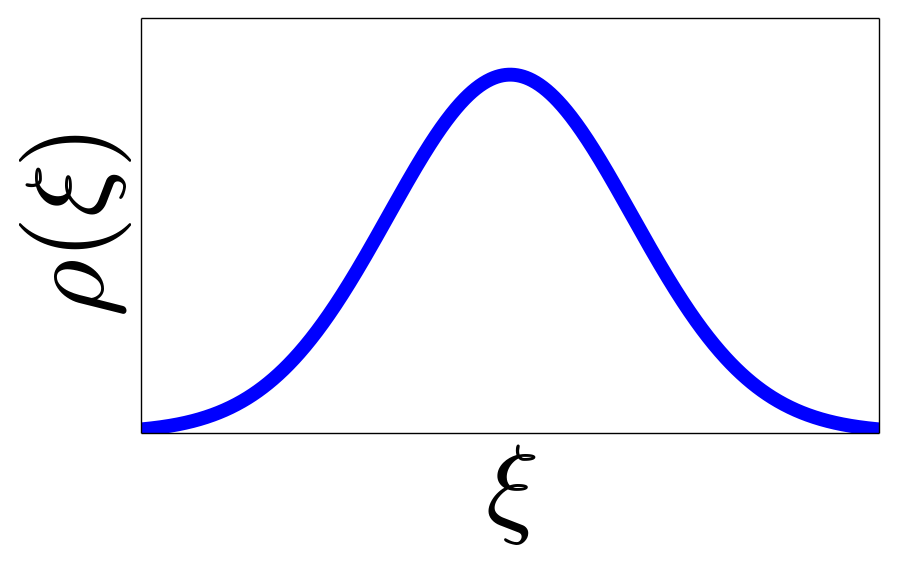
\includegraphics[width=0.9\textwidth]{ExamplePDF}\\\textbf{Input}};
    \path (CleanAirfoil)+(4,0) node (FlowSolver) [wa] {\textbf{Computation/}\\\textbf{Experiment}};
    \path (FlowSolver)+(4,0) node (Droplet) [wa] {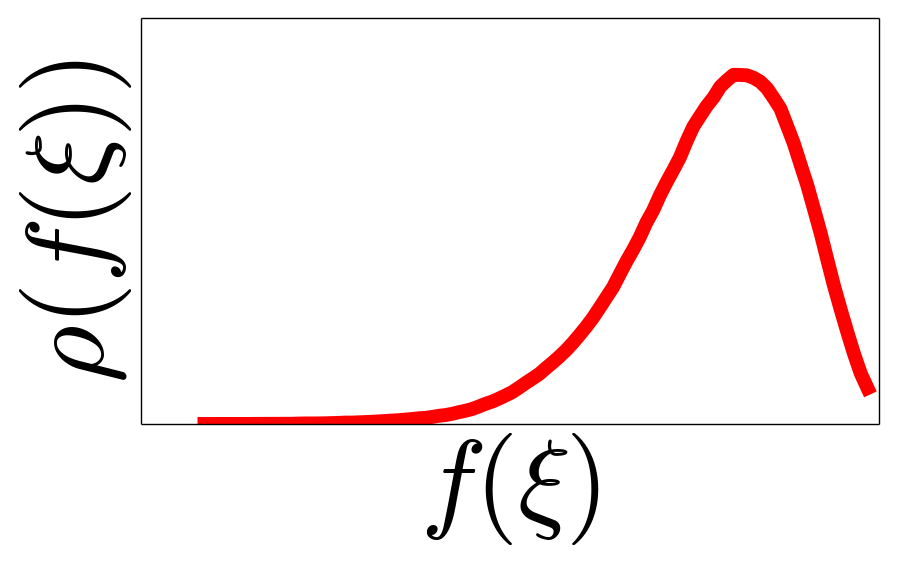
\includegraphics[width=0.9\textwidth]{ExamplePDF2}\\\textbf{Output}};

    \path [draw, ->, thick] (CleanAirfoil.east) |- node [right] {} (FlowSolver.west);
    \path [draw, ->, thick] (FlowSolver.east) -- node [right] {} (Droplet.west);
            
\end{tikzpicture}
\end{frame}
\begin{frame}
\frametitle{Polynomial Chaos Expansions (PCE)}
\label{sec-2-3}

\begin{figure}[ht]
\centering
\begin{minipage}[b]{0.45\linewidth}
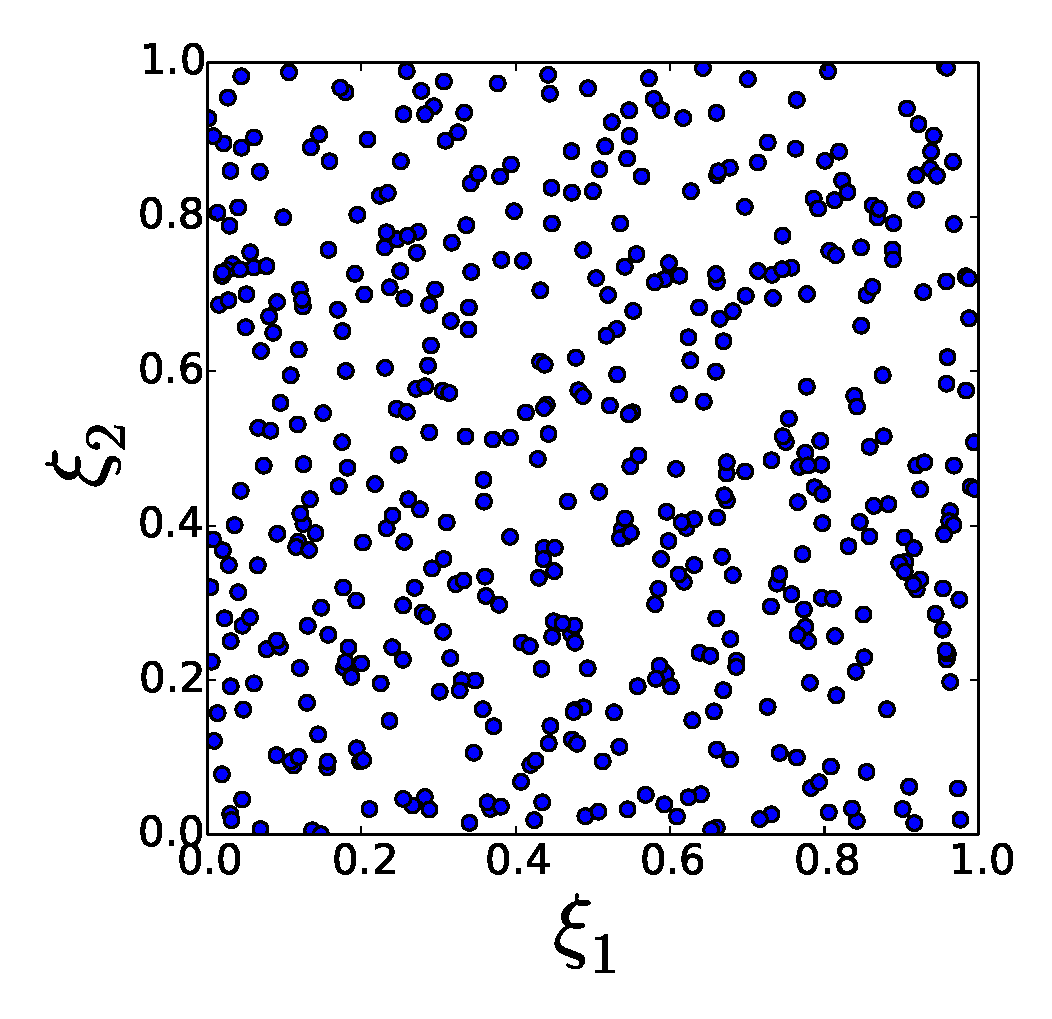
\includegraphics[width=0.7\textwidth]{MonteCarlo} \\
\centering
\textbf{Monte Carlo} \\
\begin{equation*}
  y \approx \delta(\xi - \xi_k)
\end{equation} \\
\begin{itemize}
\item Draw random samples
\item Data exist at discrete points
\end{itemize}
\end{minipage}
\begin{minipage}[b]{0.45\linewidth}
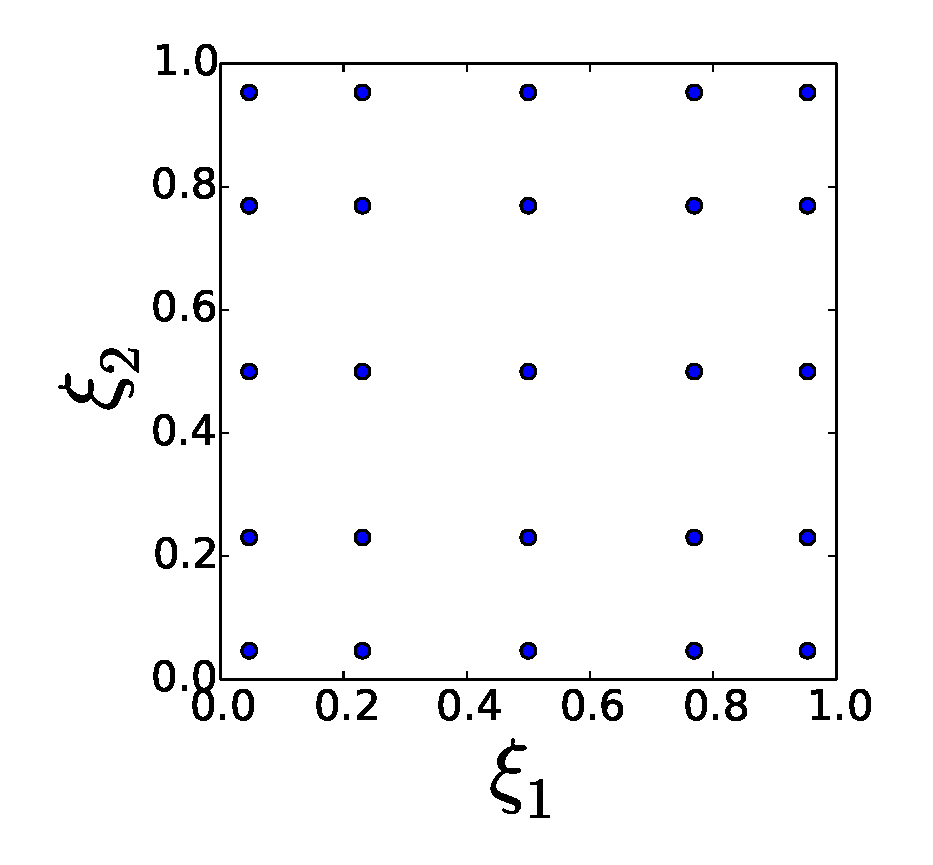
\includegraphics[width=0.7\textwidth]{QuadraturePoints} \\
\centering
\textbf{Polynomial Chaos}
\begin{equation*}
  y \approx \sum_{i}^{Q} c_i \psi_i(\xi)
\end{equation} \\
\begin{itemize}
\item Take data at collocation points
\item Construct global surrogate
\end{itemize}
\end{minipage}
\end{figure}
\end{frame}
\section{Example: Cylinder Flow}
\label{sec-3}
\begin{frame}
\frametitle{Setup}
\label{sec-3-1}

\begin{columns}[c]
\column{0.20\textwidth}
   \centering
    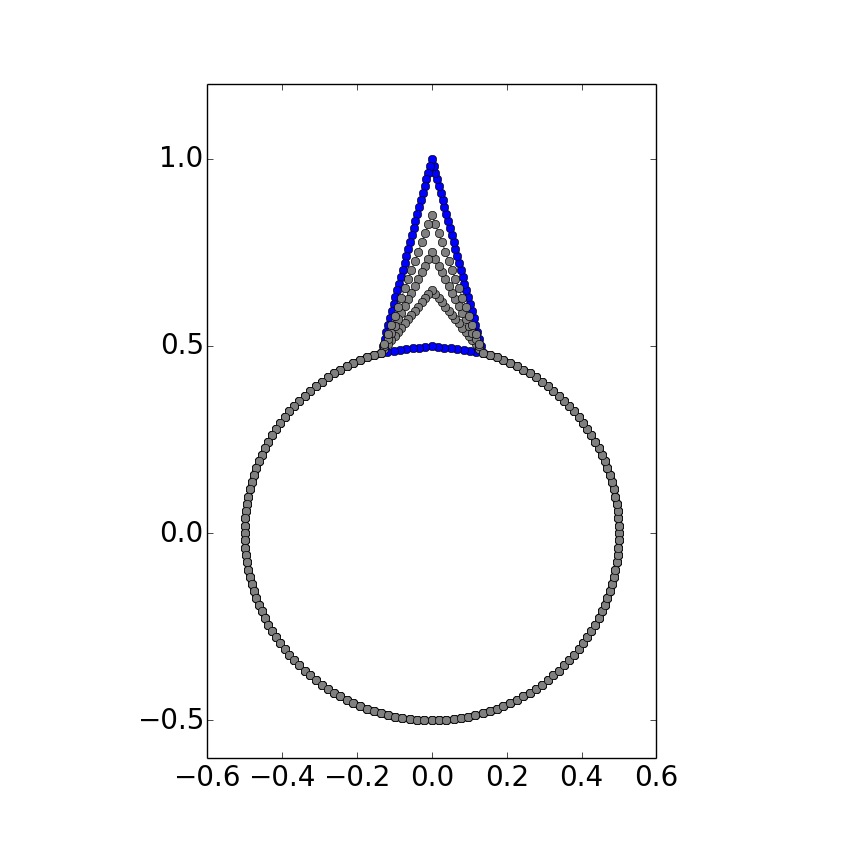
\includegraphics[width=1\textwidth]{CylinderPerturbations}   
\column{0.25\textwidth}
   \centering
    \textbf{Small Spike} \\
    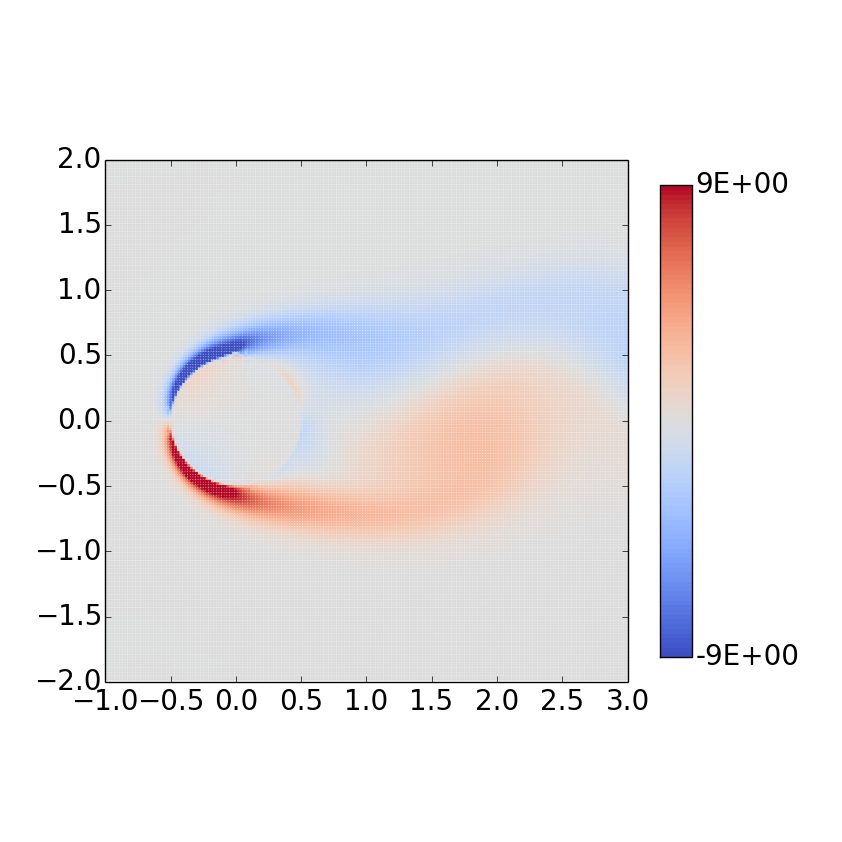
\includegraphics[width=1\textwidth]{PerturbSmallHorn}
\column{0.25\textwidth}
   \centering
    \textbf{Medium Spike} \\
    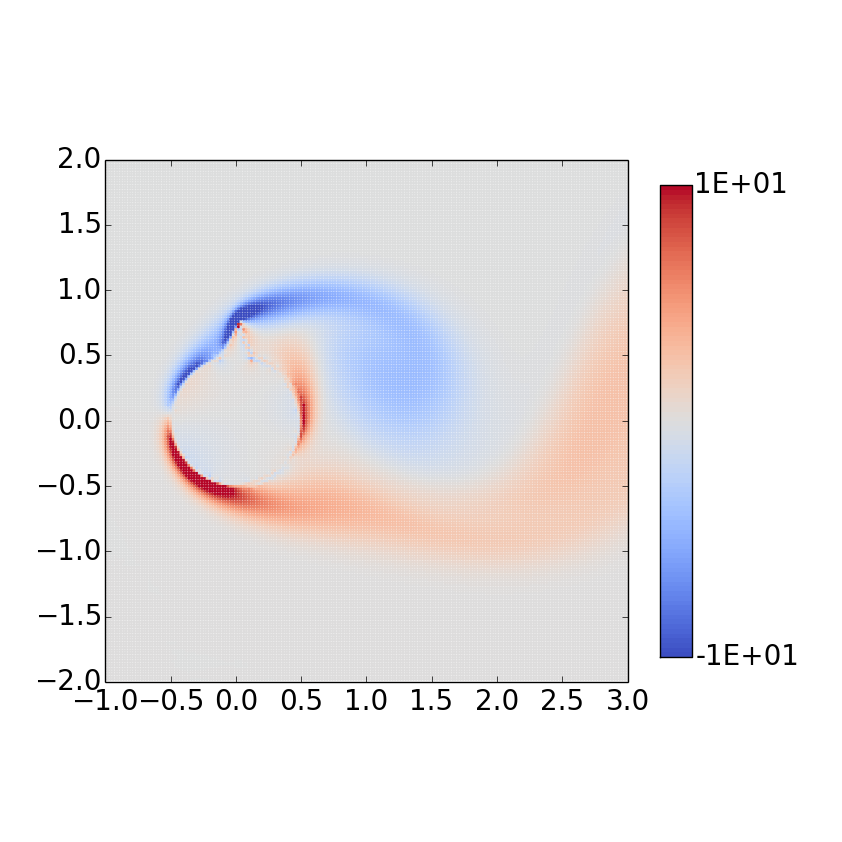
\includegraphics[width=1\textwidth]{PerturbMediumHorn}
\column{0.25\textwidth}
   \centering
    \textbf{Large Spike} \\
    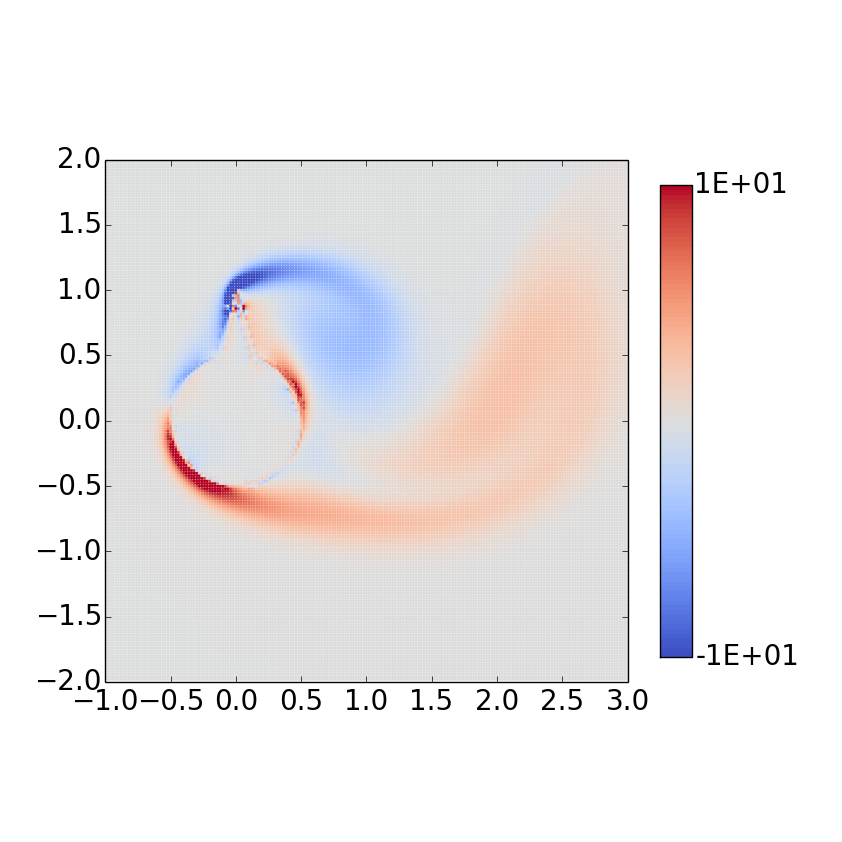
\includegraphics[width=1\textwidth]{PerturbBigHorn}
\end{columns}
\begin{itemize}
\item Assume spike height is uniformly distributed between limits shown
\item Re = 100
\item Output = wake POD modes, DMD eigenvalues
\end{itemize}
\end{frame}
\begin{frame}
\frametitle{Methodology}
\label{sec-3-2}


\fontsize{9}\selectfont
% Define the layers to draw the diagram
\pgfdeclarelayer{background}
\pgfdeclarelayer{foreground}
\pgfsetlayers{background,main,foreground}

% Define block styles used later

\tikzstyle{sensor}=[draw, fill=blue!20, text width=5em, 
    text centered, minimum height=2.5em,drop shadow]
\tikzstyle{ann} = [above, text width=5em, text centered]
\tikzstyle{wa} = [sensor, text width=10em, fill=blue!20, 
    minimum height=7em, rounded corners, drop shadow]

% Define distances for bordering
\def\blockdist{2.3}
\def\edgedist{2.5}

\begin{tikzpicture}
    \node (CleanAirfoil) [wa]  {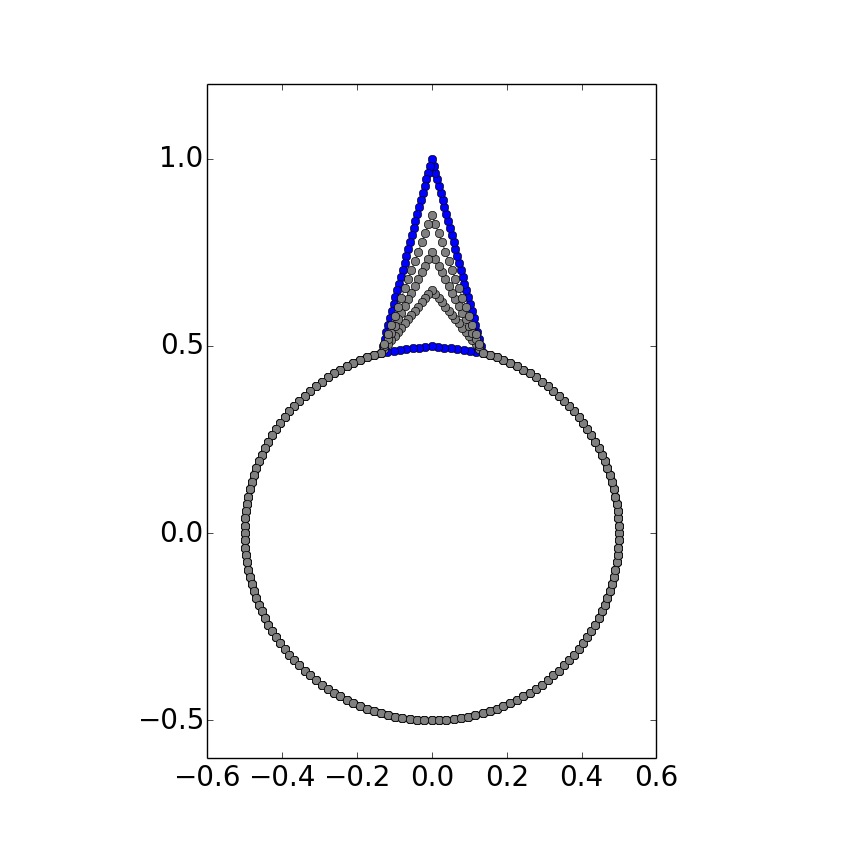
\includegraphics[width=0.9\textwidth]{CylinderPerturbations}\\\vspace{0.25cm}\textbf{Spike Height}\\ $\xi = \mathcal{U}\lbrace 0,1\rbrace$};
    \path (CleanAirfoil)+(4,0) node (FlowSolver) [wa] {\textbf{Computation (IBPM)}\\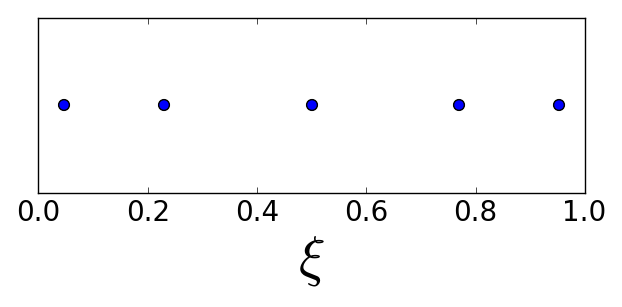
\includegraphics[width=0.8\textwidth]{QuadraturePoints1D}};
    \path (FlowSolver)+(4,0) node (Droplet) [wa] {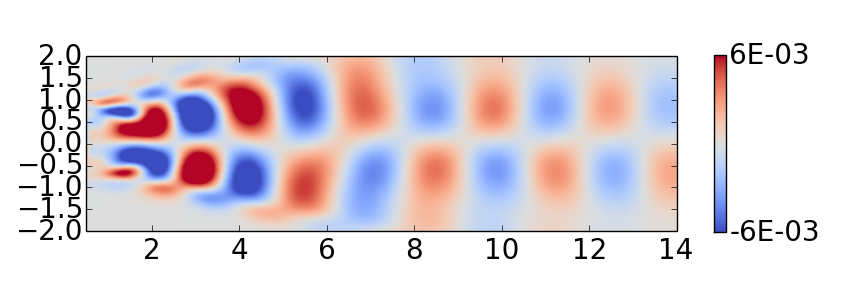
\includegraphics[width=0.9\textwidth]{POD2CompareInterp1}\\\vspace{0.25cm}\textbf{POD Modes}\\\vspace{0.2cm} $\phi(x,\xi) \approx \sum_i a_i(x) \psi_i(\xi)$};

    \path [draw, ->, thick] (CleanAirfoil.east) |- node [right] {} (FlowSolver.west);
    \path [draw, ->, thick] (FlowSolver.east) -- node [right] {} (Droplet.west);
            
\end{tikzpicture}
\end{frame}
\begin{frame}
\frametitle{Range of Flow Behavior}
\label{sec-3-3}

\begin{columns}[c]
\column{0.5\textwidth}
   \centering
    \textbf{Cylinder, Re = 100}
    \movie[width=0.9\textwidth,height=0.3\textwidth,poster,autostart,loop,borderwidth]{}{CylinderRe100.mp4} \\
    \textbf{POD Modes} \\
    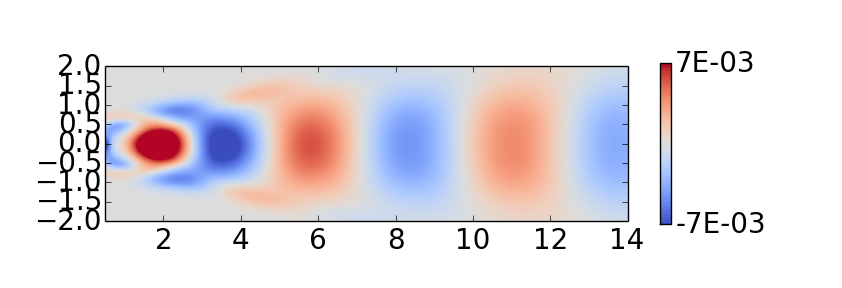
\includegraphics[width=0.9\textwidth]{CylinderRe100POD1} \\
    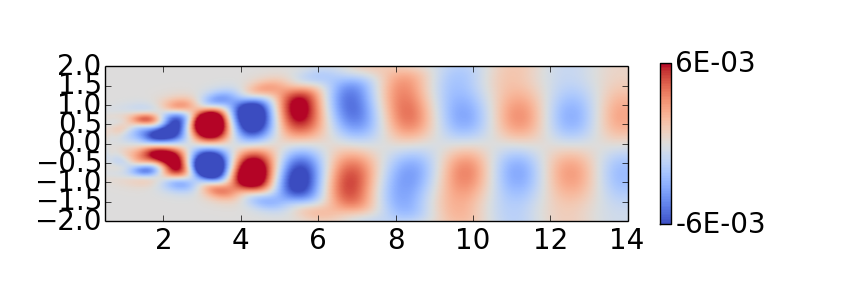
\includegraphics[width=0.9\textwidth]{CylinderRe100POD2} \\
    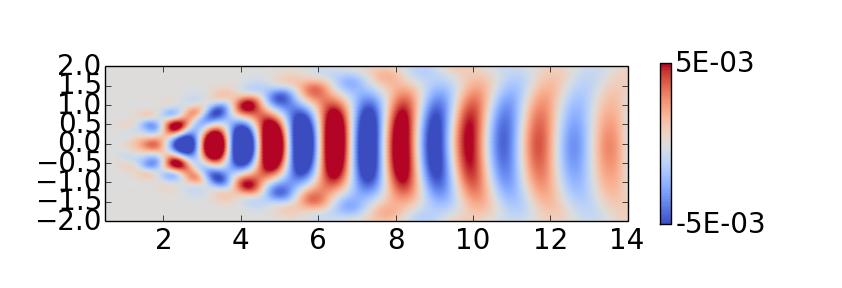
\includegraphics[width=0.9\textwidth]{CylinderRe100POD3}
\column{0.5\textwidth}
   \centering
    \textbf{Perturbed Cylinder, Re = 100}
    \movie[width=0.9\textwidth,height=0.3\textwidth,poster,autostart,loop,borderwidth]{}{PerturbCylinderRe100R1.mp4} \\
    \textbf{POD Modes} \\
    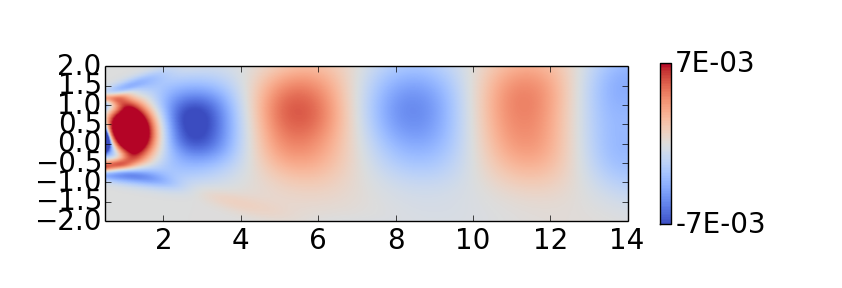
\includegraphics[width=0.9\textwidth]{PerturbRp95Re100POD1} \\
    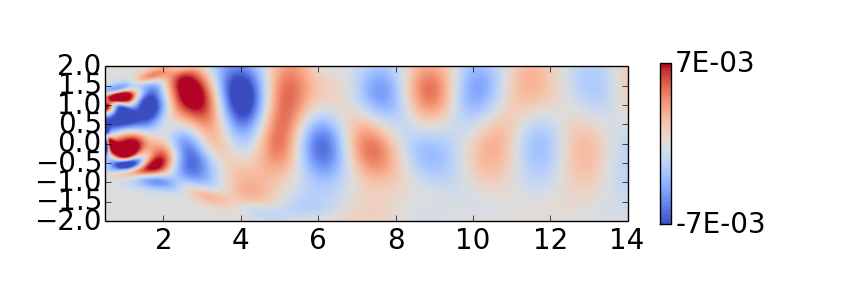
\includegraphics[width=0.9\textwidth]{PerturbRp95Re100POD2} \\
    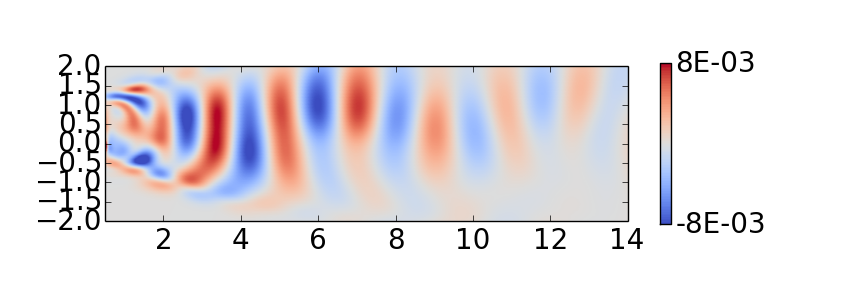
\includegraphics[width=0.9\textwidth]{PerturbRp95Re100POD3}
\end{columns}
\end{frame}
\begin{frame}
\frametitle{Explore Parameter Space}
\label{sec-3-4}

\begin{columns}[c]
\column{0.5\textwidth}
\centering
\texbf{Height = 14$\%$}\\\vspace{-0.07cm}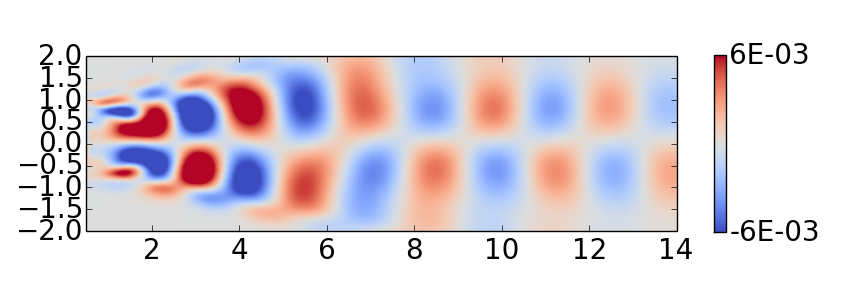
\includegraphics[width=0.95\textwidth]{POD2CompareInterp1} \\
\texbf{Height = 36$\%$}\\\vspace{-0.07cm}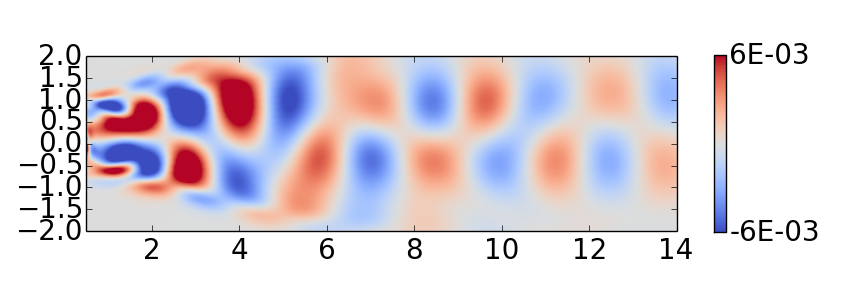
\includegraphics[width=0.95\textwidth]{POD2CompareInterp2} \\
\texbf{Height = 86$\%$}\\\vspace{-0.07cm}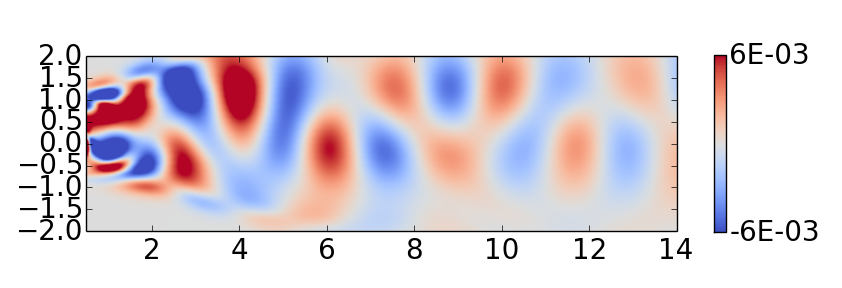
\includegraphics[width=0.95\textwidth]{POD2CompareInterp4}
\column{0.5\textwidth}
\centering
\texbf{Height = 14$\%$}\\\vspace{-0.07cm}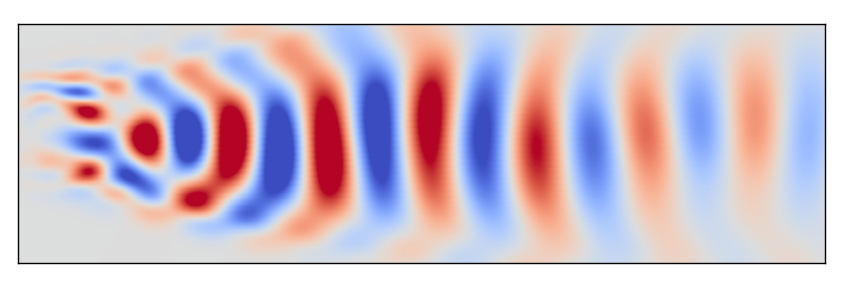
\includegraphics[width=0.95\textwidth]{POD4CompareInterp1} \\
\texbf{Height = 36$\%$}\\\vspace{-0.07cm}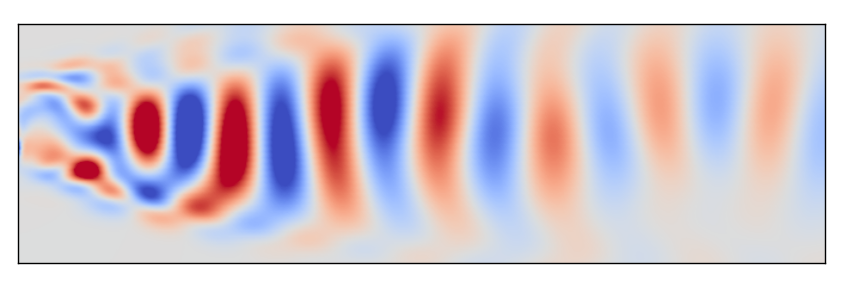
\includegraphics[width=0.95\textwidth]{POD4CompareInterp2} \\
\texbf{Height = 86$\%$}\\\vspace{-0.07cm}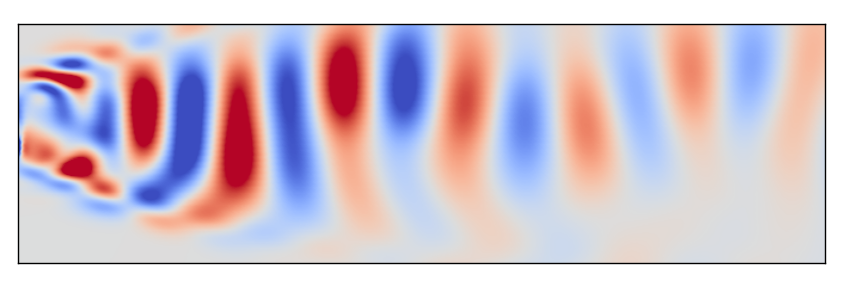
\includegraphics[width=0.95\textwidth]{POD4CompareInterp4}
\end{columns}
\begin{itemize}
\item Range from almost symmetric modes similar to cylinder to asymmetric perturbations
\end{itemize}
\end{frame}
\begin{frame}
\frametitle{Statistical Variance in Modes}
\label{sec-3-5}

\begin{columns}[c]
\column{0.5\textwidth}
\centering
\textbf{POD Mode 2} \\
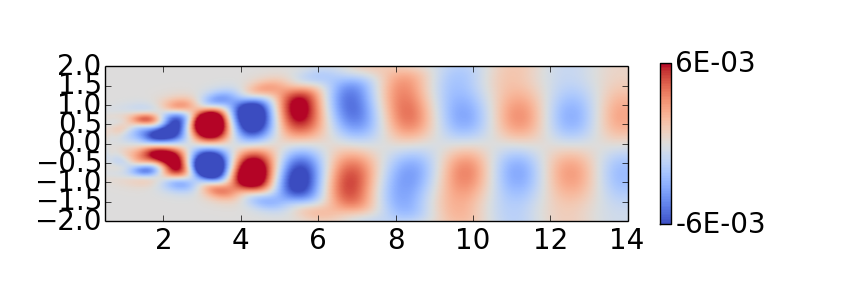
\includegraphics[width=0.95\textwidth]{CylinderRe100POD2} \\
\textbf{Statistical Variance} \\
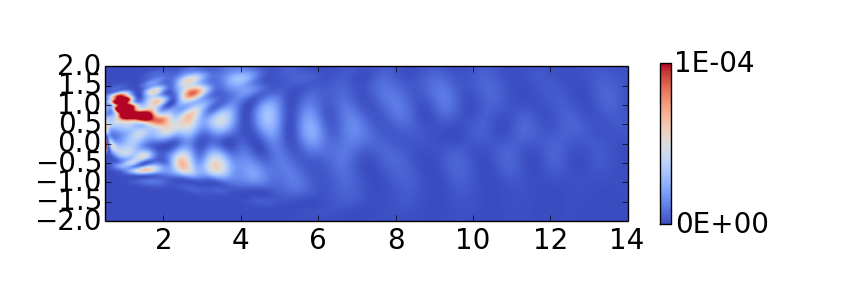
\includegraphics[width=0.95\textwidth]{VariancePOD2}
\column{0.5\textwidth}
\centering
\textbf{POD Mode 3} \\
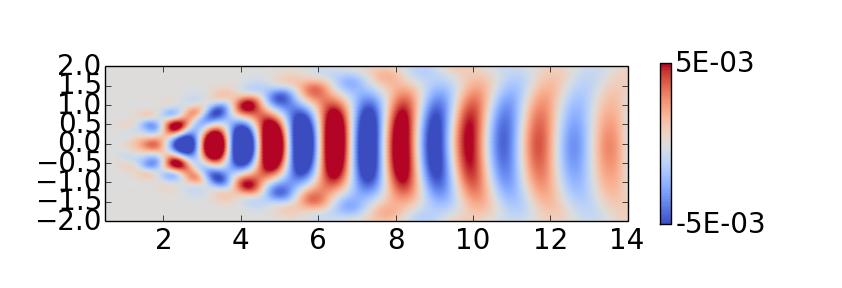
\includegraphics[width=0.95\textwidth]{CylinderRe100POD3} \\
\textbf{Statistical Variance} \\
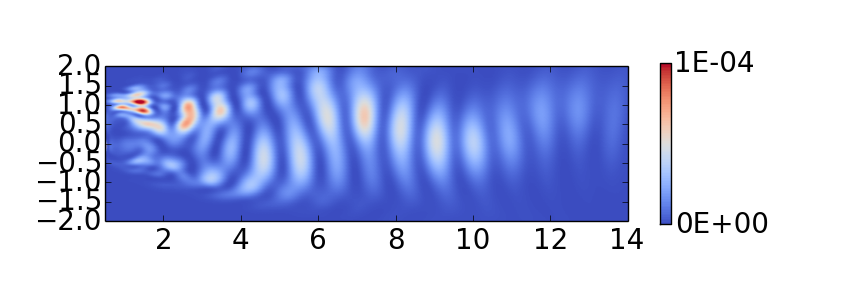
\includegraphics[width=0.95\textwidth]{VariancePOD3}
\end{columns}
\begin{itemize}
\item Can statistically sample PCE surrogate
\item Generate ensemble of cylinder spikes and associated POD modes
\item Variance shows where POD modes are most affected by spike height
\end{itemize}
\end{frame}
\begin{frame}
\frametitle{Projection Error}
\label{sec-3-6}

\begin{itemize}
\item Choose the $Q-1$ points halfway between $Q$ quadrature nodes
\item Calculate true modes and interpolated modes at $Q-1$ points
\item Compare error between true modes and interpolated modes vs. true modes and mean modes
\end{itemize}

\begin{equation*}
N(Y) \equiv max(||Y(\xi_k) - \Phi(\xi_k)||_2) \quad , \quad k = 1...Q-1
\end{equation}


\begin{center}
\begin{tabular}{|r|r|r|r}
 MODE  &  N(y_P)  &  N(\overline{y})  &  N(\overline{y})/N(y_P)  \\
\hline
    1  &    4e-3  &             3e-1  &                      75  \\
    2  &    3e-2  &             9e-1  &                      30  \\
    3  &    2e-1  &              1.2  &                       6  \\
    4  &    7e-1  &              1.5  &                       2  \\
    5  &    2e-1  &              1.8  &                       9  \\
\hline
\end{tabular}
\end{center}



\begin{itemize}
\item PCE model captures range of symmetrical to asymmetrical modes
\end{itemize}
\end{frame}
\begin{frame}
\frametitle{DMD Eigenvalues}
\label{sec-3-7}

\begin{columns}[c]
\column{0.3\textwidth}
   \centering
    \textbf{DMD Mode} \\
    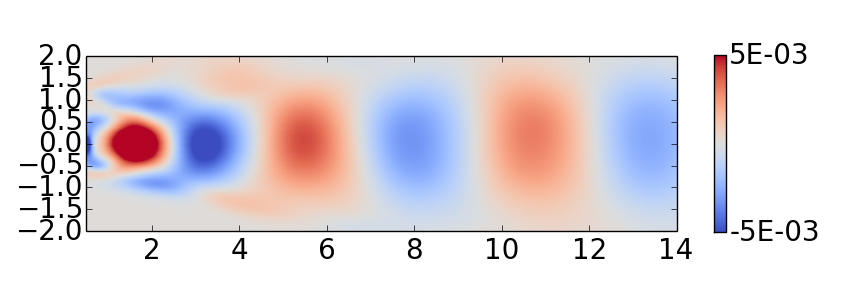
\includegraphics[width=0.9\textwidth]{DMDMode1} \\
    \textbf{Frequency Distribution} \\
    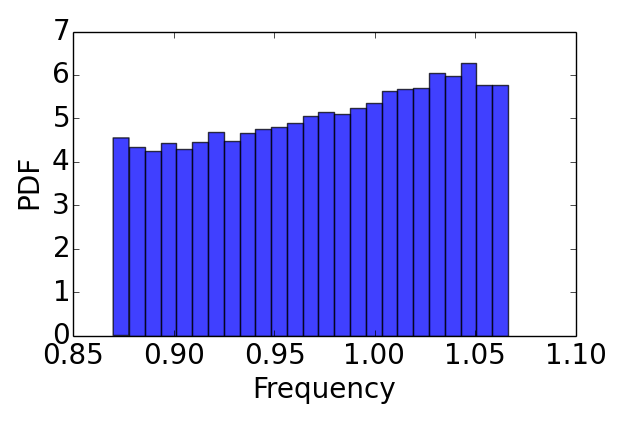
\includegraphics[width=0.9\textwidth]{PerturbDMDEigSlowPDF}
\column{0.3\textwidth}
   \centering
    \textbf{DMD Mode} \\
    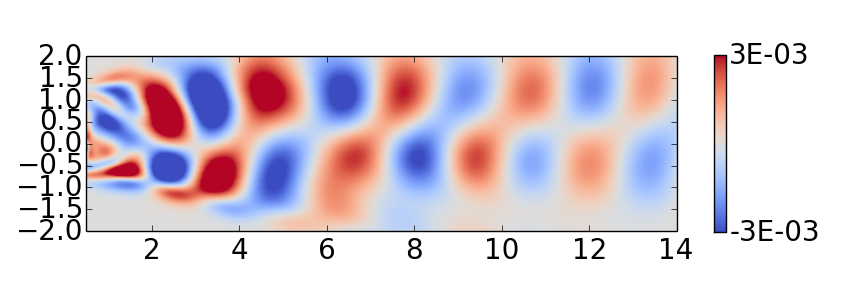
\includegraphics[width=0.9\textwidth]{DMDMode2} \\
    \textbf{Frequency Distribution} \\
    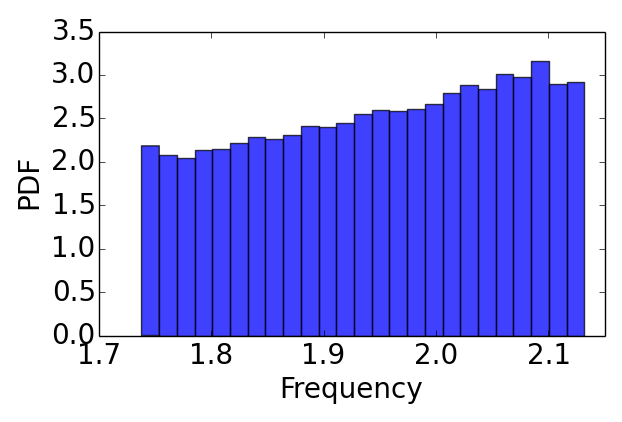
\includegraphics[width=0.9\textwidth]{PerturbDMDEigMediumPDF}
\column{0.3\textwidth}
   \centering
    \textbf{DMD Mode} \\
    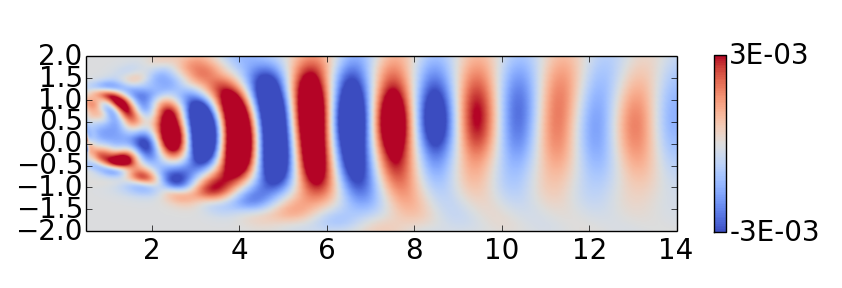
\includegraphics[width=0.9\textwidth]{DMDMode3} \\
    \textbf{Frequency Distribution} \\
    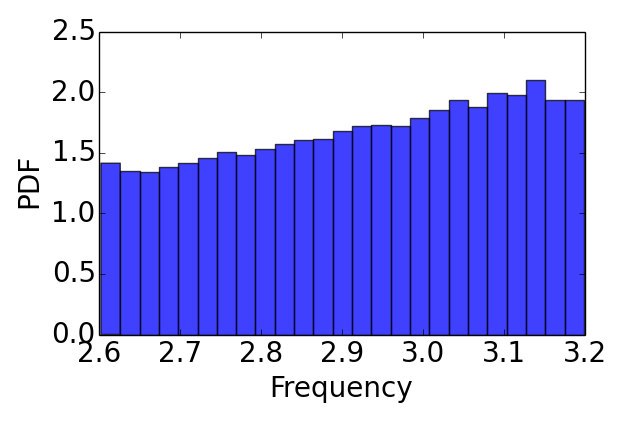
\includegraphics[width=0.9\textwidth]{PerturbDMDEigFastPDF}
\end{columns}

\begin{itemize}
\item Output is the imaginary part of DMD eigenvalues
\item Histograms are based on 10,000 Monte Carlo samples of the PCE surrogate
\item Modest deformation of uniform distribution for all frequencies
\end{itemize}
\end{frame}
\begin{frame}
\frametitle{Conclusions}
\label{sec-3-8}

\begin{itemize}
\item Uncertainty quantification techniques provide a fast, efficient, and
  accurate methodology for quantifying how low-dimensional models
  change with parametric uncertainty
\begin{itemize}
\item POD modes
\item DMD modes/eigenvalues
\end{itemize}
\item Further research
\begin{itemize}
\item Multiple parameters
\item Apply to POD Galerkin models
\end{itemize}
\end{itemize}
\end{frame}

\end{document}
